\section{Trajectory Design}

This section has as objective explore null-space motion with a planar three-link arm surgical robot, with a vital organ represented by a red circle and a green line as the trajectory. It is also important to maximize robot manipulability to avoid the vital organ, so that there is no contact. Here we are going to analyze the system with null-space and without it. 

Our main file is the matlab file "main.m", where we initialize all the data and test the system.
About the data, we used a Kp equal to 100 (to have a good performance doing the pretended trajectory), an initial position equal to $[\pi/5;\pi/4;pi/3]$, so it is similar to the robot in the image \eqref{fig:10.1}, a vertical line in $x = 1.5$ and a vital area centred at (-0.5,-0.75) with 0.3 as the value for radius. We also made some changes in our function "showRobot" because here we are working with a three-link arm and not a two-link arm.

\begin{figure}[H]
    \centering
    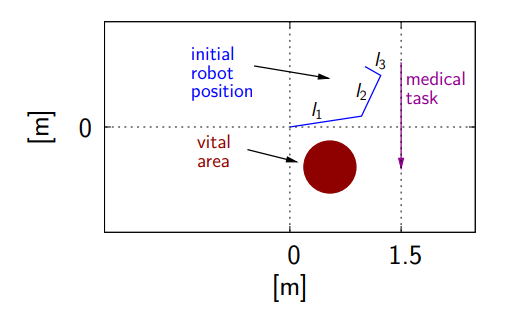
\includegraphics[width=0.49\textwidth]{imgs/10.1.png}
    \caption{Scheme for the Trajectory Design}
    \label{fig:10.1}
\end{figure}

\begin{figure}[H]
    \centering
    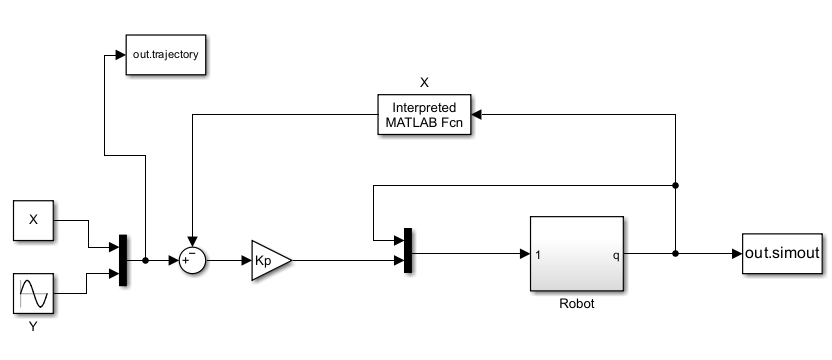
\includegraphics[width=0.49\textwidth]{imgs/10.2.png}
    \caption{Simulink for Trajectory Design}
    \label{fig:10.2}
\end{figure}

In the figure \eqref{fig:10.2} we have the simulink used for this part where we used the function "forward-kinematics".

\begin{figure}[H]
    \centering
    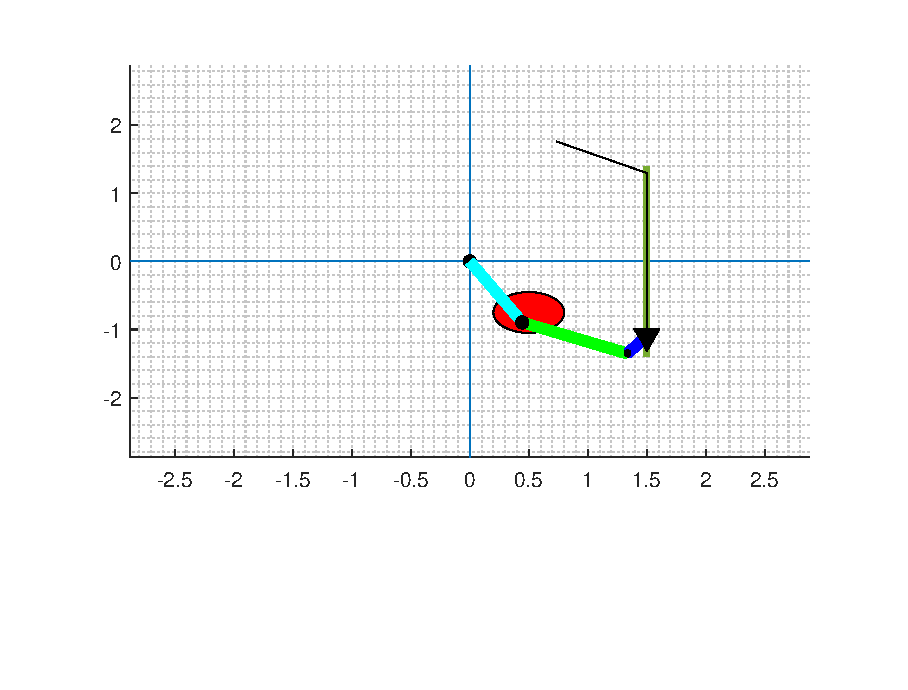
\includegraphics[width=0.49\textwidth]{imgs/10.3.eps}
    \caption{Robot simulator using simulink without null-space}
    \label{fig:10.3}
\end{figure}

\begin{figure}[H]
    \centering
    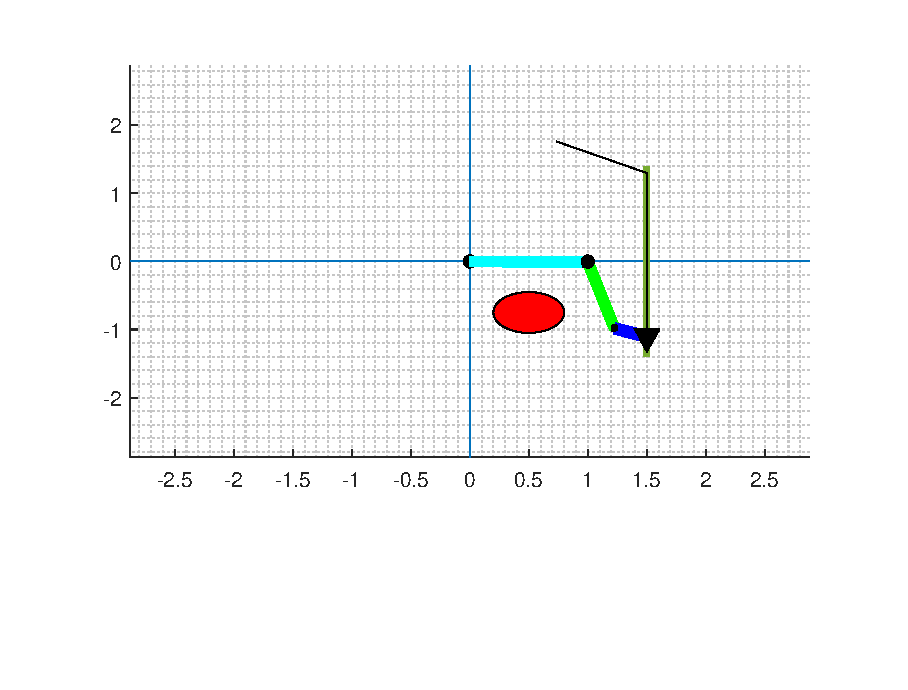
\includegraphics[width=0.49\textwidth]{imgs/10.4.eps}
    \caption{Robot simulator using simulink with null-space}
    \label{fig:10.4}
\end{figure}

In the figures \eqref{fig:10.3} \eqref{fig:10.4} we have the system without the null-space and with the null-space, respectively and for that we just changed the value $K_q$ between 0 and 10.

It can be seen in the figures that the robot behaves as it is supposed, in the figure \eqref{fig:10.3} it does the trajectory without caring about the vital area, but in the figure \eqref{fig:10.4} it does care about the vital area and changes it posture to make the trajectory correctly without touching the vital area. We can also conclude that in the figure \eqref{fig:10.3} the robot doesn't change it's position much because it does not need to avoid anything, otherwise in the figure \eqref{fig:10.4} the robot changes more it's position comparing to the initial position because it needs to avoid the vital area, so the angles of the joints, change more than without the null-space. These behaviour can be better viewed in the videos.


